% Options for packages loaded elsewhere
\PassOptionsToPackage{unicode}{hyperref}
\PassOptionsToPackage{hyphens}{url}
\PassOptionsToPackage{dvipsnames,svgnames,x11names}{xcolor}
%
\documentclass[
]{agujournal2019}

\usepackage{amsmath,amssymb}
\usepackage{iftex}
\ifPDFTeX
  \usepackage[T1]{fontenc}
  \usepackage[utf8]{inputenc}
  \usepackage{textcomp} % provide euro and other symbols
\else % if luatex or xetex
  \usepackage{unicode-math}
  \defaultfontfeatures{Scale=MatchLowercase}
  \defaultfontfeatures[\rmfamily]{Ligatures=TeX,Scale=1}
\fi
\usepackage{lmodern}
\ifPDFTeX\else  
    % xetex/luatex font selection
\fi
% Use upquote if available, for straight quotes in verbatim environments
\IfFileExists{upquote.sty}{\usepackage{upquote}}{}
\IfFileExists{microtype.sty}{% use microtype if available
  \usepackage[]{microtype}
  \UseMicrotypeSet[protrusion]{basicmath} % disable protrusion for tt fonts
}{}
\makeatletter
\@ifundefined{KOMAClassName}{% if non-KOMA class
  \IfFileExists{parskip.sty}{%
    \usepackage{parskip}
  }{% else
    \setlength{\parindent}{0pt}
    \setlength{\parskip}{6pt plus 2pt minus 1pt}}
}{% if KOMA class
  \KOMAoptions{parskip=half}}
\makeatother
\usepackage{xcolor}
\setlength{\emergencystretch}{3em} % prevent overfull lines
\setcounter{secnumdepth}{5}
% Make \paragraph and \subparagraph free-standing
\ifx\paragraph\undefined\else
  \let\oldparagraph\paragraph
  \renewcommand{\paragraph}[1]{\oldparagraph{#1}\mbox{}}
\fi
\ifx\subparagraph\undefined\else
  \let\oldsubparagraph\subparagraph
  \renewcommand{\subparagraph}[1]{\oldsubparagraph{#1}\mbox{}}
\fi


\providecommand{\tightlist}{%
  \setlength{\itemsep}{0pt}\setlength{\parskip}{0pt}}\usepackage{longtable,booktabs,array}
\usepackage{calc} % for calculating minipage widths
% Correct order of tables after \paragraph or \subparagraph
\usepackage{etoolbox}
\makeatletter
\patchcmd\longtable{\par}{\if@noskipsec\mbox{}\fi\par}{}{}
\makeatother
% Allow footnotes in longtable head/foot
\IfFileExists{footnotehyper.sty}{\usepackage{footnotehyper}}{\usepackage{footnote}}
\makesavenoteenv{longtable}
\usepackage{graphicx}
\makeatletter
\def\maxwidth{\ifdim\Gin@nat@width>\linewidth\linewidth\else\Gin@nat@width\fi}
\def\maxheight{\ifdim\Gin@nat@height>\textheight\textheight\else\Gin@nat@height\fi}
\makeatother
% Scale images if necessary, so that they will not overflow the page
% margins by default, and it is still possible to overwrite the defaults
% using explicit options in \includegraphics[width, height, ...]{}
\setkeys{Gin}{width=\maxwidth,height=\maxheight,keepaspectratio}
% Set default figure placement to htbp
\makeatletter
\def\fps@figure{htbp}
\makeatother

\usepackage{url} %this package should fix any errors with URLs in refs.
\usepackage{lineno}
\usepackage[inline]{trackchanges} %for better track changes. finalnew option will compile document with changes incorporated.
\usepackage{soul}
\linenumbers
\makeatletter
\@ifpackageloaded{tcolorbox}{}{\usepackage[skins,breakable]{tcolorbox}}
\@ifpackageloaded{fontawesome5}{}{\usepackage{fontawesome5}}
\definecolor{quarto-callout-color}{HTML}{909090}
\definecolor{quarto-callout-note-color}{HTML}{0758E5}
\definecolor{quarto-callout-important-color}{HTML}{CC1914}
\definecolor{quarto-callout-warning-color}{HTML}{EB9113}
\definecolor{quarto-callout-tip-color}{HTML}{00A047}
\definecolor{quarto-callout-caution-color}{HTML}{FC5300}
\definecolor{quarto-callout-color-frame}{HTML}{acacac}
\definecolor{quarto-callout-note-color-frame}{HTML}{4582ec}
\definecolor{quarto-callout-important-color-frame}{HTML}{d9534f}
\definecolor{quarto-callout-warning-color-frame}{HTML}{f0ad4e}
\definecolor{quarto-callout-tip-color-frame}{HTML}{02b875}
\definecolor{quarto-callout-caution-color-frame}{HTML}{fd7e14}
\makeatother
\makeatletter
\@ifpackageloaded{caption}{}{\usepackage{caption}}
\AtBeginDocument{%
\ifdefined\contentsname
  \renewcommand*\contentsname{Table of contents}
\else
  \newcommand\contentsname{Table of contents}
\fi
\ifdefined\listfigurename
  \renewcommand*\listfigurename{List of Figures}
\else
  \newcommand\listfigurename{List of Figures}
\fi
\ifdefined\listtablename
  \renewcommand*\listtablename{List of Tables}
\else
  \newcommand\listtablename{List of Tables}
\fi
\ifdefined\figurename
  \renewcommand*\figurename{Figure}
\else
  \newcommand\figurename{Figure}
\fi
\ifdefined\tablename
  \renewcommand*\tablename{Table}
\else
  \newcommand\tablename{Table}
\fi
}
\@ifpackageloaded{float}{}{\usepackage{float}}
\floatstyle{ruled}
\@ifundefined{c@chapter}{\newfloat{codelisting}{h}{lop}}{\newfloat{codelisting}{h}{lop}[chapter]}
\floatname{codelisting}{Listing}
\newcommand*\listoflistings{\listof{codelisting}{List of Listings}}
\makeatother
\makeatletter
\makeatother
\makeatletter
\@ifpackageloaded{caption}{}{\usepackage{caption}}
\@ifpackageloaded{subcaption}{}{\usepackage{subcaption}}
\makeatother
\makeatletter
\@ifpackageloaded{sidenotes}{}{\usepackage{sidenotes}}
\@ifpackageloaded{marginnote}{}{\usepackage{marginnote}}
\makeatother
\ifLuaTeX
  \usepackage{selnolig}  % disable illegal ligatures
\fi
\usepackage[]{natbib}
\bibliographystyle{plainnat}
\usepackage{bookmark}

\IfFileExists{xurl.sty}{\usepackage{xurl}}{} % add URL line breaks if available
\urlstyle{same} % disable monospaced font for URLs
\hypersetup{
  pdftitle={Solar wind discontinuities spatial evolution in the outer heliosphere},
  pdfauthor={Zijin Zhang; Anton V. Artemyev; Vassilis Angelopoulos; Shi Chen},
  colorlinks=true,
  linkcolor={blue},
  filecolor={Maroon},
  citecolor={Blue},
  urlcolor={Blue},
  pdfcreator={LaTeX via pandoc}}

\journalname{JGR: Space Physics}

\draftfalse

\begin{document}
\title{Solar wind discontinuities spatial evolution in the outer heliosphere}

\authors{Zijin Zhang\affil{1}, Anton V. Artemyev\affil{1}, Vassilis Angelopoulos\affil{1}, Shi Chen\affil{1}}
\affiliation{1}{University of California, Los Angeles, }
\correspondingauthor{Zijin Zhang}{zijin@ucla.edu}


\begin{abstract}
We present a study of the spatial evolution of solar wind discontinuities in the outer heliosphere using data from the Juno spacecraft during its cruise phase. We identify and analyze the properties of the discontinuities at different radial distances from the Sun. By differentiating the temporal effect (correlated with solar activity) and spatial variations (correlated with radial distance), we find that (1) the normalized occurrence rate of IDs drops with the radial distance from the Sun, following a \(1/r\) law; (2) The thickness of IDs increases with the radial distance from the Sun, but after normalization to the ion inertial length, the thickness of IDs decreases; (3) The current intensity of IDs decreases with the radial distance from the Sun, but after normalization to the Alfven current, the current intensity of IDs increases.
\end{abstract}




\section{Introduction}\label{introduction}

Rapid variations in interplanetary magnetic fields, commonly recognized as solar wind magnetic discontinuities \citep{colburnDiscontinuitiesSolarWind1966}, embody localized transient rotations or jumps of the magnetic field. Considered important for efficient plasma heating, they carry the most intense currents found in the solar wind and obserrved throughout the heliosphere from inner heliosphere \citep{liuCategorizingMHDDiscontinuities2022} to the heliosheath \citep{burlagaCurrentSheetsHeliosheath2011}. Theoretical models \citep[\citet{medvedevDissipativeDynamicsCollisionless1997}]{lerchePropagationMagneticDisturbances1975} and MHD simulations \citep[\citet{grecoStatisticalAnalysisDiscontinuities2009}, \citet{yangFormationRotationalDiscontinuities2015}]{grecoIntermittentMHDStructures2008} suggest that the formation and destruction of discontinuities are closely related to the nonlinear dynamics of Alfvén waves and/or Alfvénic turbuluence. These nonlinear processes can create significant isolated disturbances to the otherwise adiabatic evolution of the solar wind flow (?Reference?) and host many processes, including magnetic reconnection (?Reference?) and Fermi acceleration of particles \citep{wentzelMotionMagneticDiscontinuities1964}. Moreover, they contribute significantly to the magnetic fluctuation spectra \citep{borovskyContributionStrongDiscontinuities2010} and can affect space weather \citep{tsurutaniReviewInterplanetaryDiscontinuities2011}. Therefore, the study of the spatial evolution of solar wind discontinuities is important for understanding the dynamics of the solar wind and test the local generation mechanism of discontinuities. However, previous study of solar wind discontinuities evolution \citep{sodingRadialLatitudinalDependencies2001} in the outer heliosphere were rarely in conjunction with measurements closer to the Sun. Moreover, the intervals in their study spread over multiple solar cycles though they are selected during solar activity minimum. Thus it is presently unclear whether their frequency and properties are the result of solar variability or due to the natural evolution of the discontinuities during their propagation and interaction with the ambient solar wind.

The goal of our paper is to investigate, statistically, discontinuities at different radial distance in the outer heliosphere to obtain a understanding of their formation and evolution. Our methodology involves integrating Juno measurements \citep{connerneyJunoMagneticField2017} between \(1\) and \(5\) AU with those at \(1\) AU to distinguish temporal effect and spatial variations by examining the discontinuity characteristics at two radial distances simultaneously.

First, the missions, instruments and data used are listed. Then, we briefly describe the method used to identify the discontinuities and the model used to estimate the plasma state at Juno location due to the lack of plasma data during its cruise phase. Finally, we present the results of the spatial evolution of the discontinuities with respect to their characteristics (spatial scales and current density), and discuss the implications of our findings.

\section{Methods}\label{methods}

\begin{itemize}
\tightlist
\item
  We use \citep{liuMagneticDiscontinuitiesSolar2022} method to identify IDs, which has better compatibility for the IDs with minor field changes.
\item
  Then the minimum variance analysis is applied to each ID event to obtain the boundary normal (LMN) coordinate and extract IDs' features.
\end{itemize}

\begin{figure*}

\begin{minipage}{0.33\linewidth}
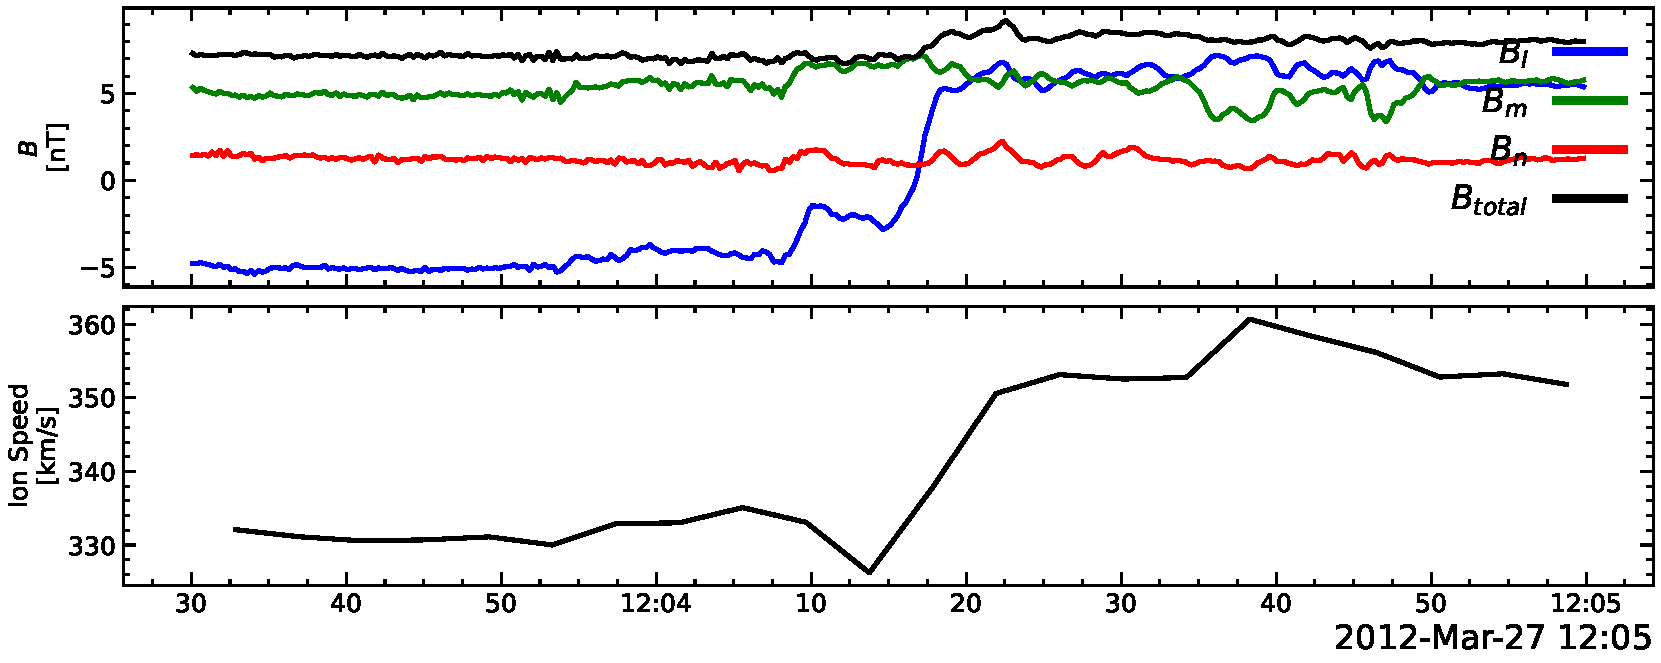
\includegraphics{figures/examples/artemis_id_example.pdf}\end{minipage}%
%
\begin{minipage}{0.33\linewidth}
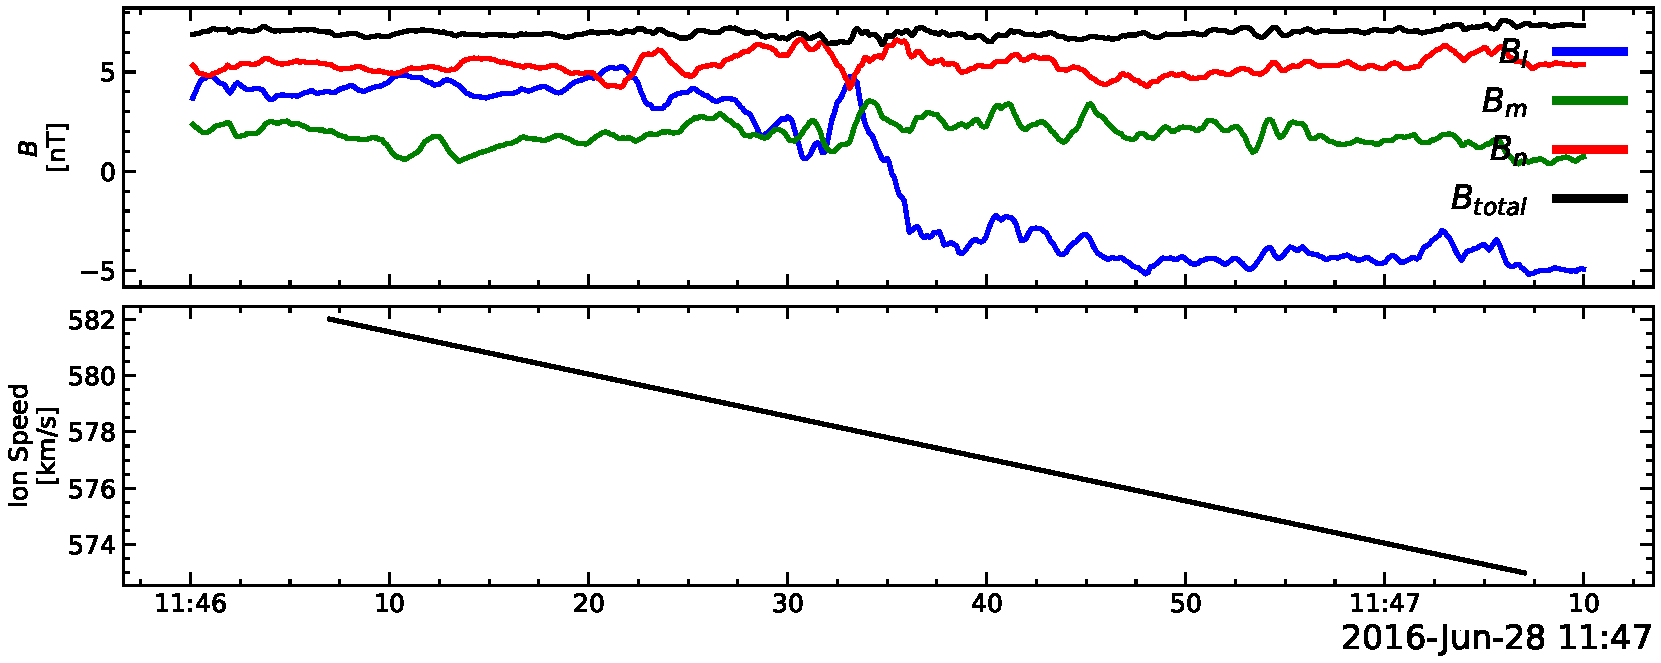
\includegraphics{figures/examples/stereo_id_example.pdf}\end{minipage}%
%
\begin{minipage}{0.33\linewidth}
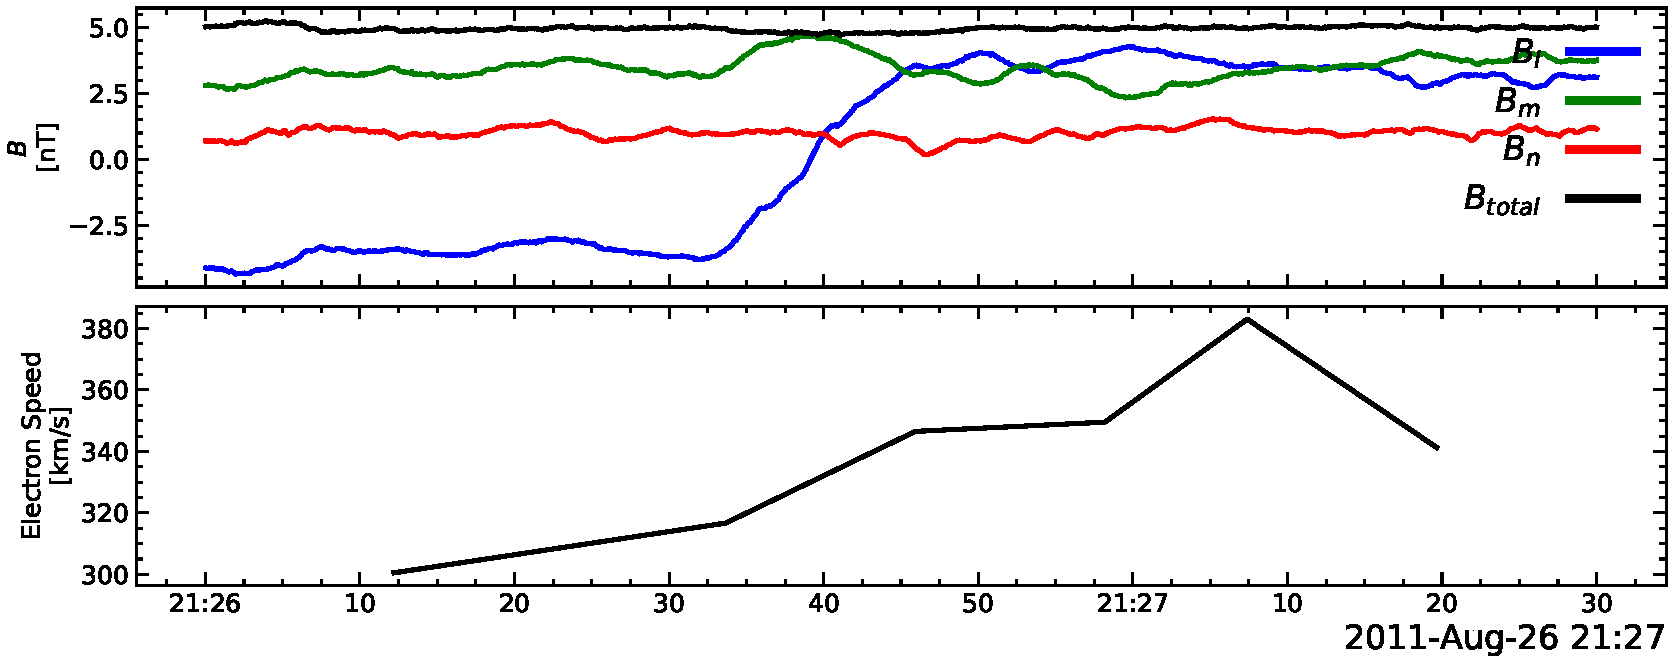
\includegraphics{figures/examples/wind_id_example.pdf}\end{minipage}%

\caption{\label{fig-examples}Examples of IDs from ARTEMIS, STEREO, and Wind}

\end{figure*}%

\subsection{ID identification (limited feature extraction / anomaly detection)}\label{id-identification-limited-feature-extraction-anomaly-detection}

Traditional methods for ID identification, such as the criteria of

\begin{itemize}
\tightlist
\item
  Burlaga \& Ness (1969; B-criterion) : a directional change of the magnetic field larger than 30° during 60 s
\item
  Tsurutani \& Smith (1979; TS-criterion) : \(|ΔB|/|B| \geq 0.5\) within 3 minutes
\end{itemize}

Mostly rely on magnetic field variations with a certain time lag. B-criterion has, as its main condition.

In their methods, the IDs below the thresholds are artificially abandoned. Therefore, identification criteria may affect the statistical results, and there is likely to be a discrepancy between the findings via B-criterion and TS- criterion.

Liu's method : The first two conditions guarantee that the field changes of the IDs identified are large enough to be distinguished from the stochastic fluctuations on magnetic fields, while the third is a supplementary condition to reduce the uncertainty of recognition.

\[ 
\textrm{Index}_1 = \frac{\sigma(\vec{B})}{Max(\sigma(\vec{B}_-),\sigma(\vec{B}_+))} 
\]

\[
\textrm{Index}_2 = \frac{\sigma(\vec{B}_- + \vec{B}_+)} {\sigma(\vec{B}_-) + \sigma(\vec{B}_+)}
\]

\[
\textrm{Index}_3 = \frac{| \Delta \vec{B} |}{|B_{bg}|}
\]

\[ 
\textrm{Index}_1 \ge 2, \textrm{Index}_2 \ge 1, \textrm{Index}_3 \ge 0.1 
\]

\subsection{Solar Wind Model}\label{solar-wind-model}

Sadly, JUNO does not provide plasma data during the cruise phase, so to estimate the plasma state we will use MHD model.

We are using \href{http://csem.engin.umich.edu/MSWIM2D/}{Michigan Solar WInd Model 2D (MSWIM2D)}, which models the solar wind propagation in 2D using the BATSRUS MHD solver. \citet{keeblerMSWIM2DTwodimensionalOuter2022}

Some key points about the model

\begin{itemize}
\tightlist
\item
  Representing the solar wind in the ecliptic plane from 1 to 75 AU
\item
  2D MHD model, using the BATSRUS MHD solver
\item
  Inclusion of neutral hydrogen (important for the outer heliosphere)
\item
  Inner boundary is filled by time-shifting in situ data from multiple spacecraft
\end{itemize}

For model validation part, please see \href{notebooks/20_model.ipynb}{JUNO Model Report}.

\section{Conclusion}\label{conclusion}

\begin{itemize}
\tightlist
\item
  We have collected 5 years of solar wind discontinuities from JUNO, aMIS and STEREO.
\item
  We have developed a pipeline to identify solar wind discontinuities. (Modular, Performant, Scalable)
\item
  The normalized occurrence rate of IDs drops with the radial distance from the Sun, following \(1/r\) law.
\item
  The thickness of IDs increases with the radial distance from the Sun, but after normalization to ion inertial length, the thickness of IDs decreases.
\item
  The current intensity of IDs decrease with the radial distance from the Sun, but after normalization to the Alfven current , the current intensity of IDs increases.
\end{itemize}

\section{Figures}\label{figures}

\begin{figure}

\centering{

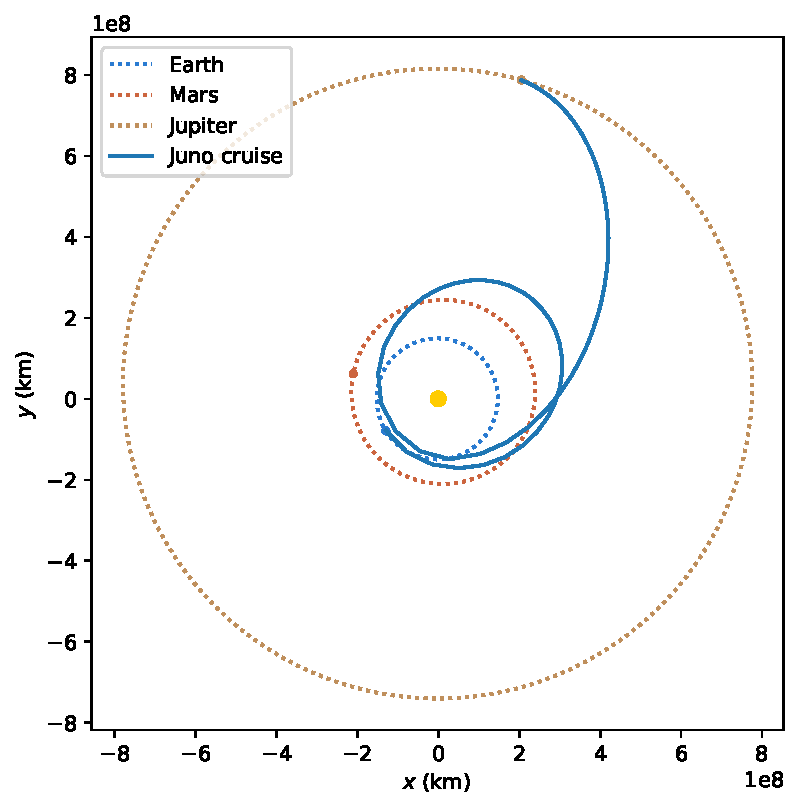
\includegraphics{figures/juno_orbit_white.pdf}

}

\caption{\label{fig-orbit}Juno orbit}

\end{figure}%

\begin{figure*}

\begin{minipage}{0.33\linewidth}
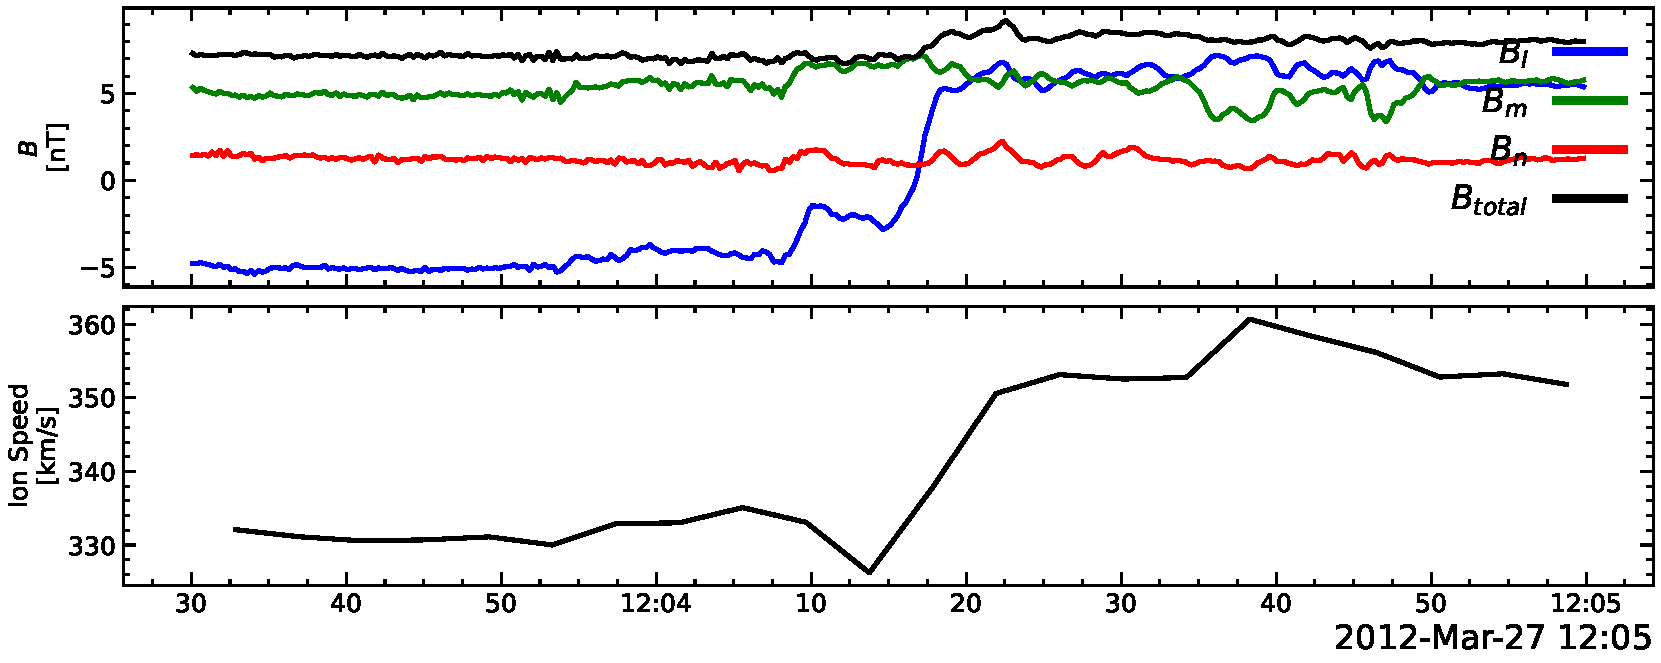
\includegraphics{figures/examples/artemis_id_example.pdf}\end{minipage}%
%
\begin{minipage}{0.33\linewidth}
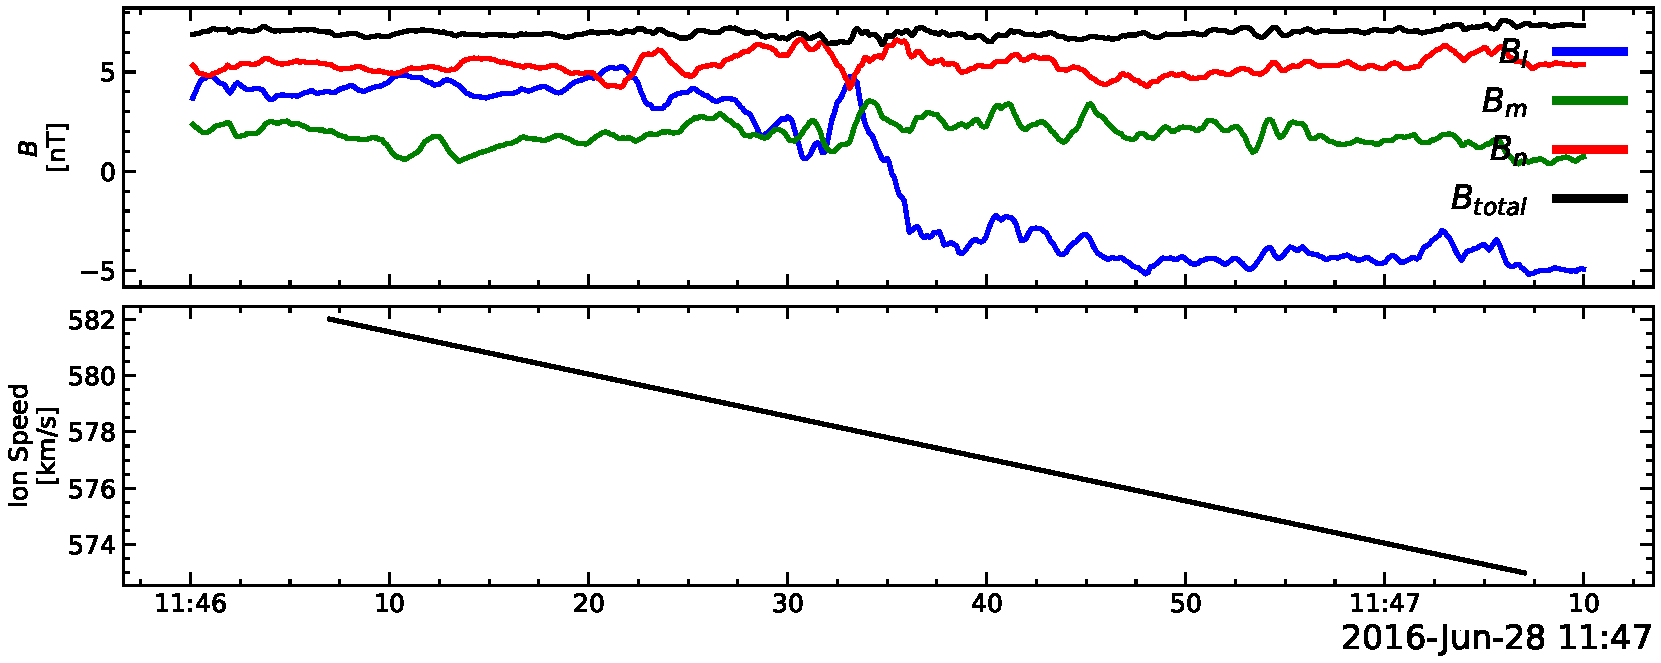
\includegraphics{figures/examples/stereo_id_example.pdf}\end{minipage}%
%
\begin{minipage}{0.33\linewidth}
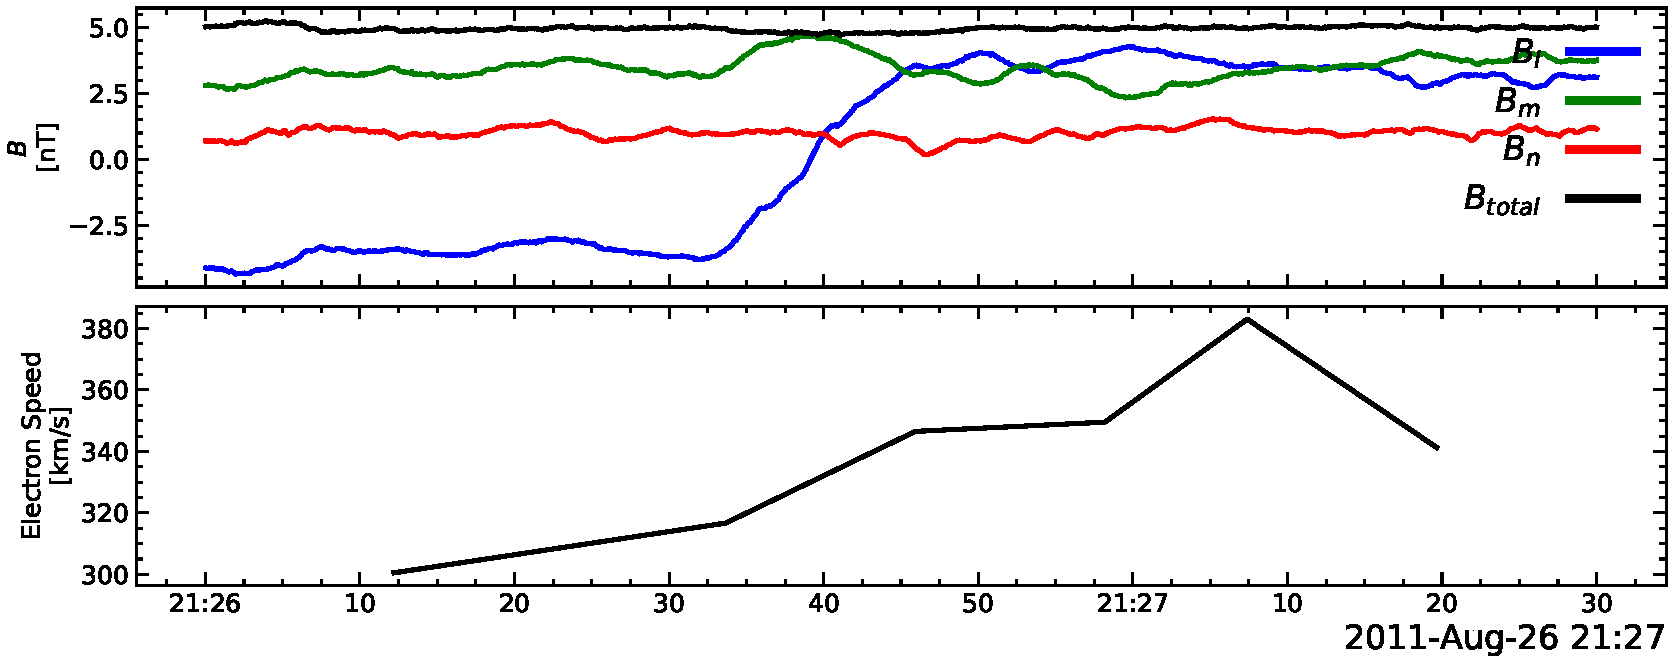
\includegraphics{figures/examples/wind_id_example.pdf}\end{minipage}%

\caption{\label{fig-examples}Examples of IDs from ARTEMIS, STEREO, and Wind}

\end{figure*}%

\begin{figure}

\centering{

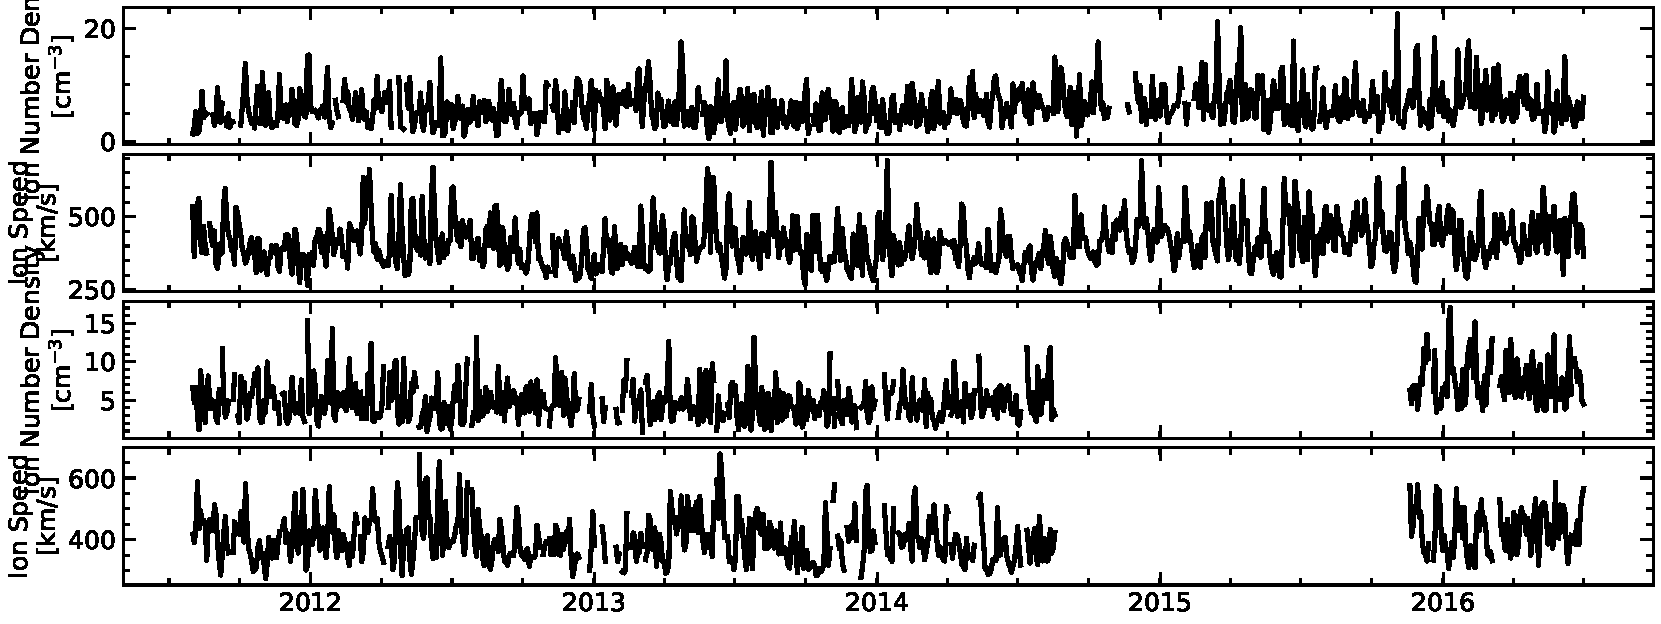
\includegraphics{figures/omni_overview.pdf}

}

\caption{\label{fig-overview}Near-Earth's solar wind plasma data during JUNO cruise phase}

\end{figure}%

Overview of the solar wind at 1 AU

{\marginnote{\begin{footnotesize}For code, see \href{notebooks/20_omni_overview.ipynb}{noteboook}.\end{footnotesize}}}

\begin{figure}

\centering{

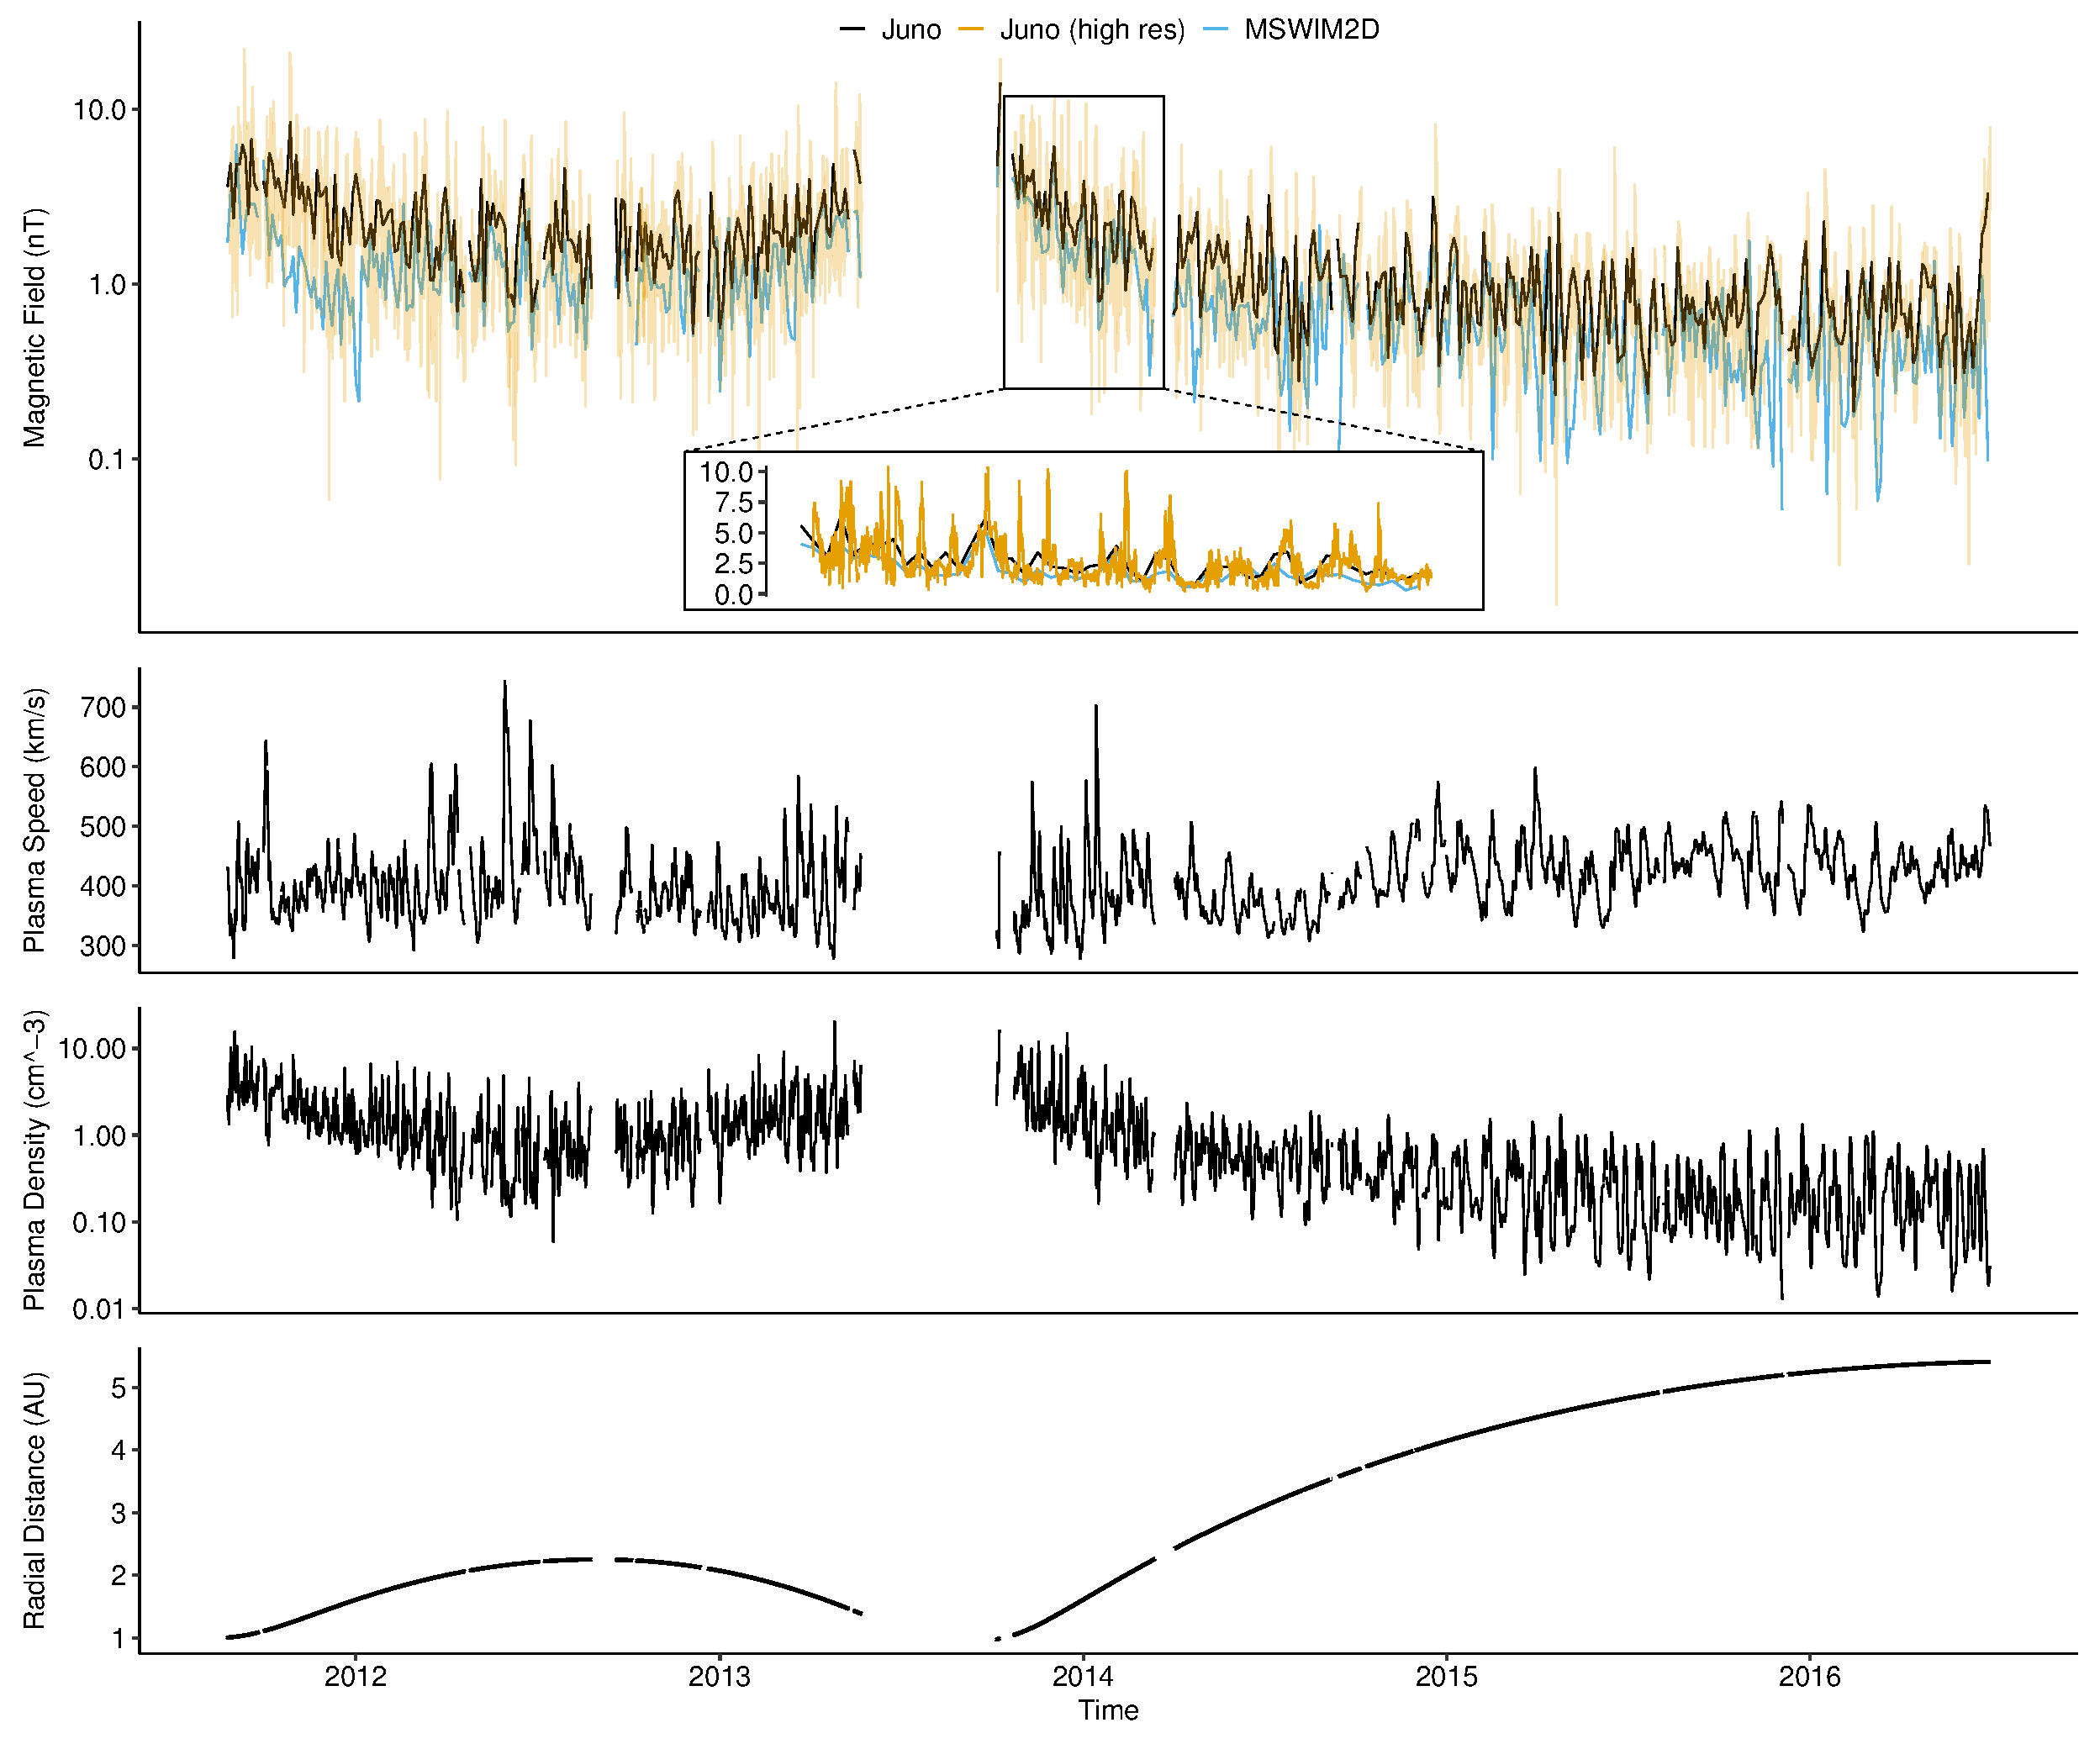
\includegraphics{figures/model/juno_model_validation_full.pdf}

}

\caption{\label{fig-modelValidation}Model validation}

\end{figure}%

\begin{figure}

\centering{

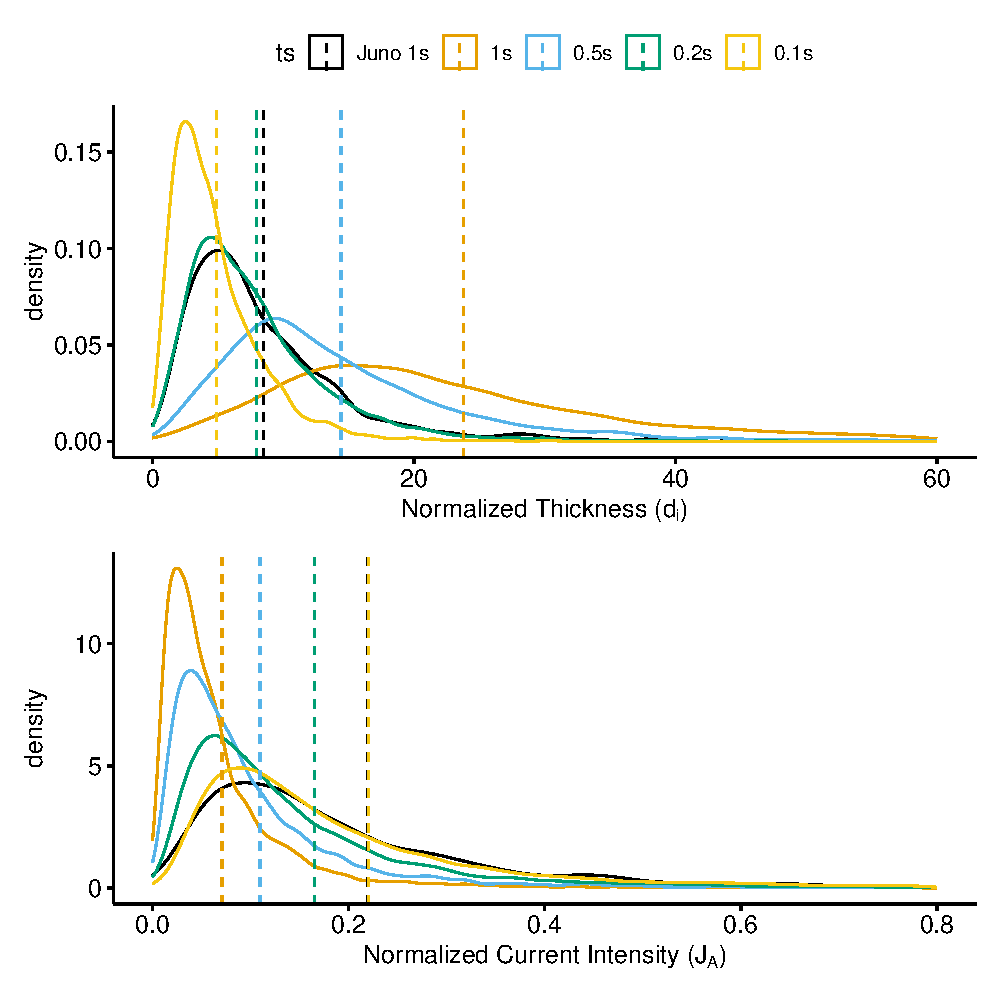
\includegraphics{figures/ts_effect.pdf}

}

\caption{\label{fig-tsEffect}Effect of the time resolution on the discontinuity properties}

\end{figure}%


  \bibliography{files/bibexport.bib,../research.bib,files/bibliography/full\_anton.bib,files/bibliography/addon\_anton.bib}


\end{document}
